\chapter{Anexo}
\label{Desarrollo}
Con el fin de poder ejecutar los modelos ANNs desarrollados y calcular el balance hídrico de la cuenca, 
se han creado dos aplicaciones REST APIs utilizando la librería flask de python \cite{flask}. La idea 
es que mediante la correcta estructuración de los datos de entrada necesarios para la ejecución de los modelos, estos se puedan ejecutar en diferentes 
cuencas.
Para esto se han creado diferentes clases y métodos en python que constituyen el core de la API, estos métodos o recursos se hacen 
accesibles a través de la interfaz de la API, en la que se exponen los métodos y las URLs disponibles para acceder 
y/o manipular cada uno de ellos.


El proceso que se ha seguido para crear esta API es el siguientes:


\begin{itemize}
    \item En primer lugar se ha construido una base de datos relacional que contiene los descriptores las cuencas hidrográficas (Fig. \ref{BD}), así como 
   también todos los datos referentes a los diferentes usos de agua. Esta base de datos fue realizada con el software PostgreSQL  un sistema 
   de código abierto de administración de bases de datos del tipo relacional cuyas consultas  se basan en SQL\cite{PostgretSQL}.
   Por otro lado las series temporales que actúan como inputs de los modelos no admiten consultas relacionales y por lo tanto 
   se han almacenado de forma separada en archivos de excel en un directorio local. 
   \item Una vez estructurados los datos en sus diferentes formatos, se ha desarrollado una serie de métodos en python para hacer todo tipo de consultas,
   agregaciones, actualizaciones, y borrado de los datos. Para esto se utilizó la librería psycopg2, una de las librerías más populares que sirven para 
   integrar el lenguaje de PostgreSQL en python y permite crear métodos que hagan consultas en la base de datos creada con dicho software.
   \item El tercer paso es crear una API que contenga todos los métodos que faciliten el acceso a los datos, entre los métodos creados se destacan 
   métodos que 
   permiten recorrer la navegación de la cuenca, encontrar para una cuenca dada,  las cuencas aguas arriba que vierten en ella,
    todas las demandas y aportaciones de agua, etc (Fig. \ref{BD}).
    \item Una vez creara la API que contiene los métodos que permiten la consulta de la base de datos y las series temporales, 
    se ha creado otra aplicación que ejecuta los modelos desarrollados (Fig. \ref{MELCA}). Para esto se ha creado una clase python, que posee varios métodos, 
    que ejecutan los modelos, y calculan el balance hídrico de la cuenca. Para esto es necesario utilizar la librería
    la librería request que permite hacer peticiones HTTP POST y GET a la base de datos que contiene las tablas con las series temporales y 
    los descriptores necesarios para la ejecución de los modelos.
    \item Por último, una vez que se ha accedido a todos los datos necesarios para ejecutar los modelos que simulan/predicen los caudales
    naturales de las cuencas, y los datos asociados a todas las demandas y aportaciones de agua, 
    se procede a  calcular el balance hídrico de la cuenca siguiendo los pasos:
    \begin{enumerate}
        \item para una subcuenca dada, se agregan los resultados de las simulaciones de caudal aguas arriba siguiendo el cauce de 
        navegación de la cuenca,
        \item se averiguan todas las demandas que toman agua de dicha cuenca y todas las demandas que retornan agua a la misma,
        \item se calcula el balance como: $q_{ac}-q_{dem}+q_{ret}$, donde $q_{ac}$ el caudal natural agregado aguas arriba, $q_{dem}$ el caudal 
        agregado de todas las demandas y $q_{ret}$ el retorno total de todas las demandas.
    \end{enumerate}  
\end{itemize}


\begin{figure}[h!]
    \begin{center}
      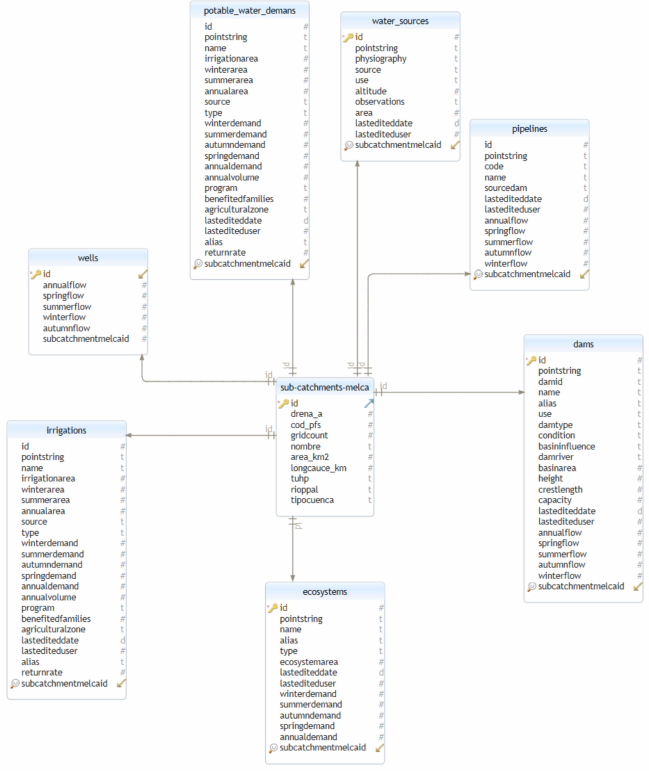
\includegraphics[height=7.in]{Figures/BD_diagram.png}
      \caption{ Base de datos relacional con los descriptores de las componentes de una cuenca hidrográfica. }
      \label{BD}
    \end{center}
  \end{figure}

  \begin{figure}[h!]
    \begin{center}
      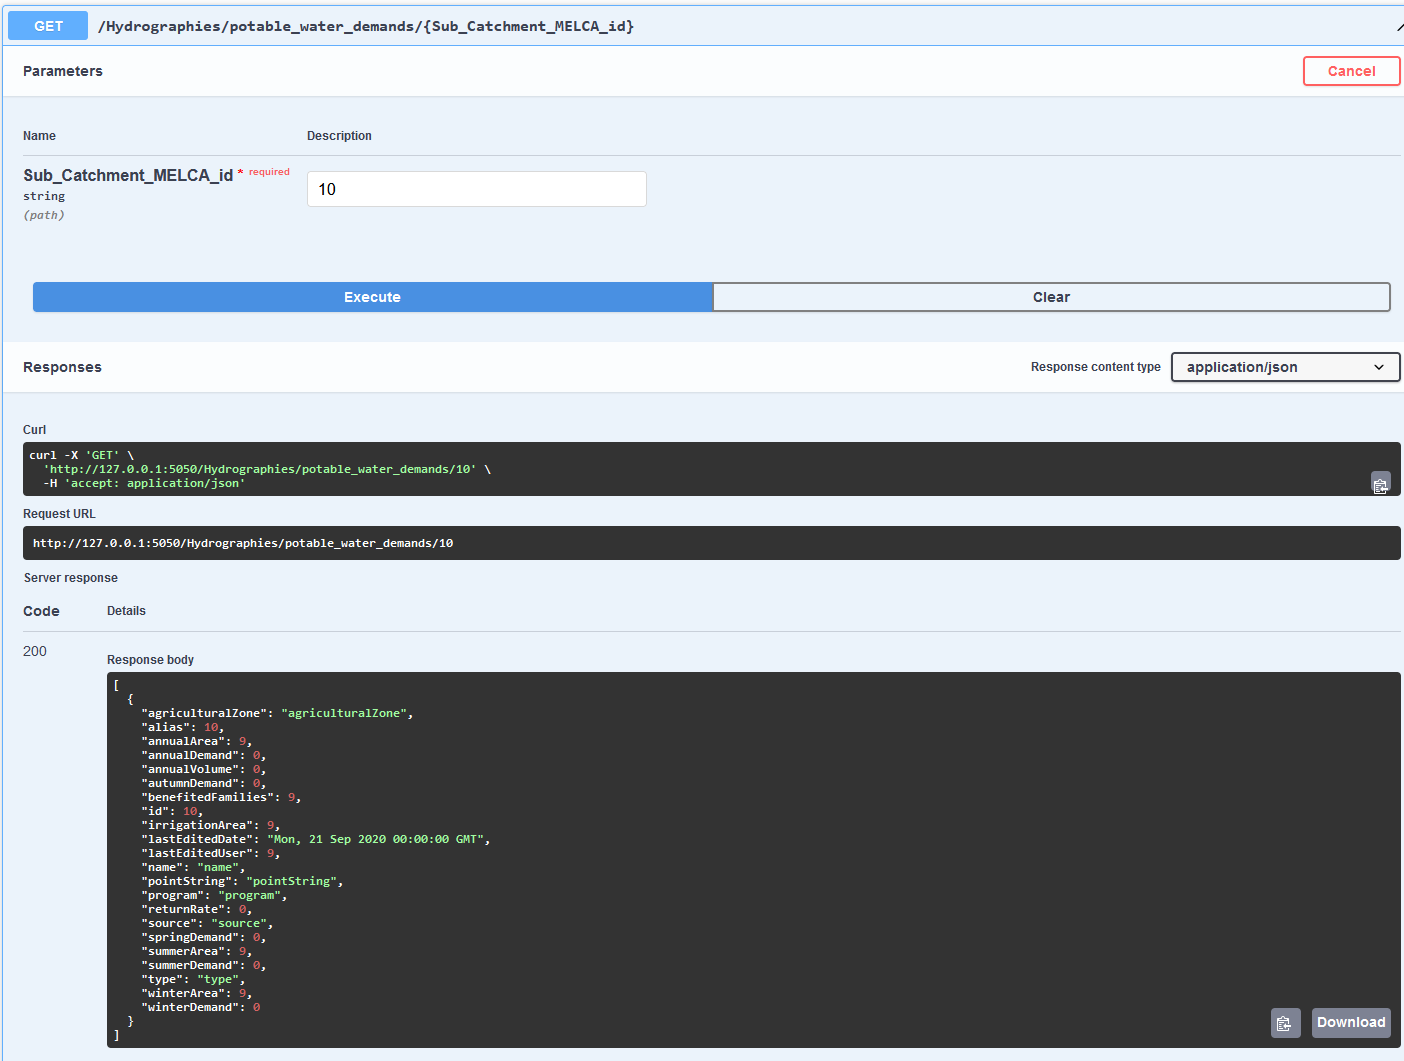
\includegraphics[height=4.in]{Figures/potable water demands.PNG}
      \caption{ Ejemplo de consulta de uno de los métodos de la API que contiene la base de datos. }
      \label{BD}
    \end{center}
  \end{figure}

  

  \begin{figure}[h!]
    \begin{center}
      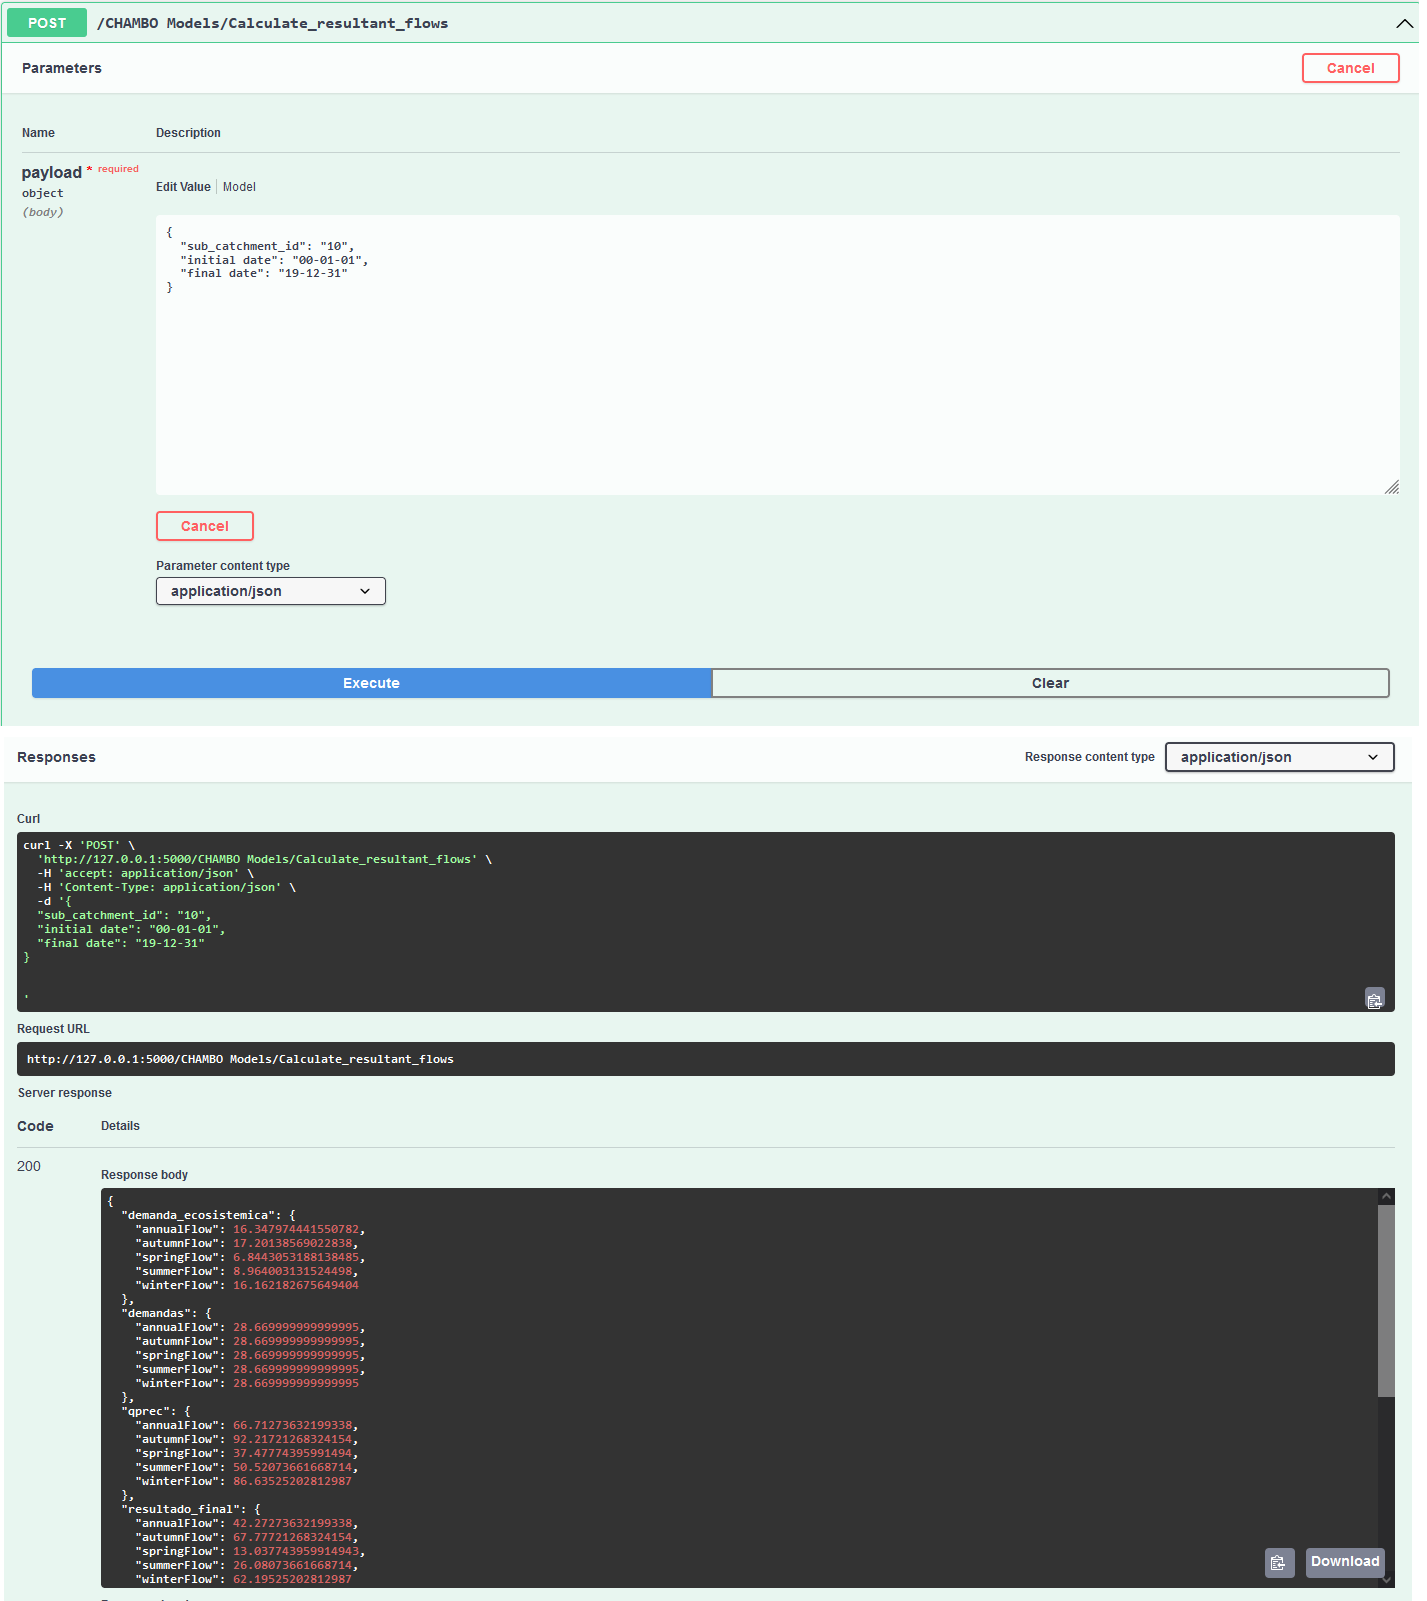
\includegraphics[height=7.in]{Figures/consulta_MELCA.png}
      \caption{ Ejemplo de consulta del método que calcula el balance hídrico de la cuenca. }
      \label{MELCA}
    \end{center}
  \end{figure}


% por un lado se ha construido una base de datos relación



% , así como los parámetros necesesarios para ejecutar los modelos 

% Para esto se han desarrollado dos aplicaciones con la librería flask de python. Una aplicación que contienen una serie de métodos que permiten 
% hacer una consulta de los descriptores de las cuencas hidrográficas y las series temporales necesarias para ejecutar los modelos. 

% Para esto se ha creado una base de datos relacional (Fig. ---) que contiene los descriptores de las cuencas, así como tambien
% todos los datos referentes a los diferentes usos de agua utilizando el software postgresql,  un sistema de código abierto de 
% administración de bases de datos del tipo relacional, aunque también es posible ejecutar consultas que sean no relaciones. 
% En este sistema, las consultas relacionales se basan en SQL, mientras que las no relacionales hacen uso de JSON.

% y la librería psycopg2,
% una de las librerías más populares que sirven para integrar el lengaje de PostgreSQL en python y permite crear métodos que hagan consultas en la base
% de datos creada con dicho software.

% Los métodos creados permiten consultar, agregar, eliminar y actualizar los diferentes componentes de CHRC, 
% así como obtener información de la estructura de la cuenca permitiendo reconstruir el recorrido del agua entre los diferentes cauces.

% En la figura ---se muestran a modo de ejemplo algunos de los métodos de la API creada. 
% El objetivo de crear esta api es el de facilitar la ejecución de los modelos en otras cuencas hidrográficas.

% Una vez creara la API que contiene la base de datos, se ha creado otra aplicacion, tambien con python y con la 
% libreria flaskj que contiene dos metodos, uno para ejecutar el modelo MELCA y otro para ejecutar el modelo LSTM1 PCA. 
% Para esto se ha utilizado la libreria request para hacer consultas a la api que contiene la base de datos y los inputs de los modelos.

% En esta aplicacion se ha utilzado la libreria de pandas para convertir los resultados de las consultas de la BD a datasets
% de panda y facilitar operaciones como la agregacion de las cuencas aguas arriba siguiendo la estructura de la red, 
% agilizar las consultas de las demandas de agua y poder calcular el equilibrio hidrico de todo el sistema.

